\chapter{Terminología DevOps}\label{ch:devops}
%************************************************
Al haber consolidado la metodología de desarrollo SCRUM en los capítulos anteriores (\ref{sec:metodologia}), sabemos que dicha metodología pertenece a un ámbito de desarrollo iterativo e incremental, donde el proyecto se planifica en diversos bloques temporales. Debido a esto es muy frecuente que el equipo de desarrollo tenga numerosas entregas, ya que debe proporcionar una versión incrementada en cada iteración, esto también se suele denominar como despliegue.

\vspace{0.3cm}

Generalmente para proporcionar un despliegue el equipo de desarrollo se divide en dos ámbitos o departamentos. El primero tiene la función de desarrollo o la propia codificación de la aplicación, reconocido como «development» o «Dev» del inglés. El segundo se encarga de la parte operacional o el gestionado de versiones y la parte física del despliegue, reconocido también como «operations» o «Ops». \cite{redahat-devops}

\vspace{0.3cm}

El problema más usual es que ambos departamentos tienden a estar separados, por lo que el flujo de comunicación tiende a fallar y a tener retrasos a la hora de proporcionar el despliegue. Bajo esta premisa, surge una solución en 2009 denominada como \textit{DevOps}, la cual tiene como propósito unificar estos dos ámbitos \cite{redahat-devops}

\vspace{0.3cm}

\begin{figure}[H]
    \centering
    \myfloatalign
    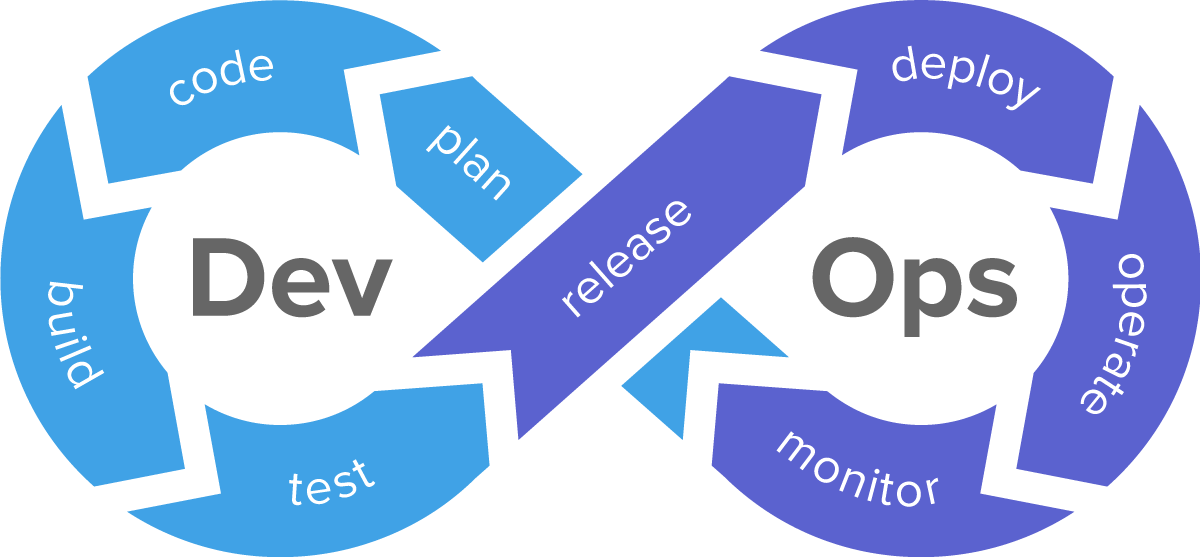
\includegraphics[width=0.7\textwidth]{gfx/devops-explicativo.png}
    \caption[Imagen explicativa del concepto DevOps]{Imagen explicativa del concepto DevOps \cite{azure-devops}.}\label{gfx:devops-explicativo}
\end{figure}

A groso modo, \textit{DevOps} trata de romper estos silos organizativos establecidos y intenta centrarse en la mejora de calidad de la entrega al cliente. Para ello, \textit{DevOps} se apoya en tres principios o también llamadas «the three ways», las cuales se deben implementar de forma consecutiva. \cite{ilimit-devops}

\begin{enumerate}
    \item\textit{Mejora del flujo de entrega}: consiste en general valor al producto, mediante entregas del software de una forma temprana y periódica. Tratando de dividir los procesos en tareas más pequeñas o automatizando todas las tareas que sean posibles, con esto se consigue un aumento del flujo de trabajo global, ya que en este caso un proceso no ralentiza a otro. \\
    Un ejemplo de este principio puede ser la ejecución de tests u otras operaciones cada vez que haya cambios en el repositorio del código fuente.
    \item\textit{Buen uso de los ciclos de feedback}: consiste en el uso de la retroalimentación con el objetivo de optimizar los procesos, es decir, cada vez que se lleve a cabo una entrega conviene tener un \textit{feedback} rápido y constante. Con esto se consigue que los ciclos de retroalimentación obtengan la información necesaria para que las correcciones se puedan aplicar de manera continua. \\
    Un ejemplo de ello puede ser la monitorización del sistema y la comunicación ante la detección de errores.
    \item\textit{Asentar el aprendizaje y la mejora continua}: se centra en aplicar todo lo anteriormente realizado y aprendido para implementar un sistema de mejora continua. De esta manera se consigue innovar el producto, pero sin criminalizar los errores mediante el aprendizaje y las pruebas continuas. \\
    Un ejemplo puede llegar a ser usar programas extremos de pruebas o prestaciones.
\end{enumerate}

\section{Control de Versiones}
Una de las principales plataformas en sacar provecho de los flujos o vías que se han explicado anteriormente es GitHub. Aunque el objetivo principal de la plataforma no sea este, sino alojar proyectos mediante el control de versiones Git y la creación de código fuente. Debido a esto, a la hora de alojar el código fuente del proyecto, es usual llegar a incidir sobre las diferentes vías de \textit{DevOps}. \cite{github-manual}

\vspace{0.3cm}

Mi aplicación también ha aprovechado esta plataforma y el uso de la herramienta Git. La principal ventaja a la hora de usar Git es la capacidad de controlar los cambios en el código fuente del proyecto y tener múltiples versiones en caso de posible retorno a una versión previa, un funcionamiento parecido a un historial. Por otro lado, la principal ventaja a la hora de usar GitHub es poder compartir el código con una comunidad y la integración continua en el repositorio ante cualquier cambio.

\vspace{0.3cm}

De esta manera, las plataformas de servicio (\ac{PaaS}) como Heroku o Vercel pueden encargarse del despliegue continuo ante cualquier cambio del repositorio del proyecto y de la monitorización. Gracias a esto mejoramos el flujo de la entrega continuo y sus ciclos de \textit{feedback}, ya que también se envía un correo ante un despliegue correcto o fallido.

\section{Implementación Back-end}

Para la gestión, virtualización y empaquetado de dependencias en Python del proyecto se ha elegido la herramienta \textit{Poetry}. Esta herramienta nos facilitará la portabilidad de nuestro proyecto, ya que declara todas las dependencias y gestiona las actualizaciones en un archivo. Mediante este archivo se puede repetir y distribuir la instalación en diferentes máquinas. Además, dicho gestor nos ayudará a cumplir las diferentes vías de \textit{DevOps}. \cite{poetry-manual}

\vspace{0.2cm}

\begin{table}[H]
\centering
\small
\begin{tabular}{| >{\centering\arraybackslash}m{0.6in} >{\centering\arraybackslash}m{0.8in} |}
\hline
\multicolumn{1}{|p{0.6in}|}{\cellcolor{RoyalBlue}\textbf{Terminal:}} & \multicolumn{1}{p{0.8in}|}{\textit{poetry install}} \\ \hline
\end{tabular}
\caption[Instalación del proyecto]{Instalación del proyecto.}
\end{table}

\begin{table}[H]
\centering
\small
\begin{tabular}{| >{\centering\arraybackslash}m{0.6in} >{\centering\arraybackslash}m{2.9in} |}
\hline
\multicolumn{1}{|p{0.6in}|}{\cellcolor{RoyalBlue}\textbf{Terminal:}} & \multicolumn{1}{p{2.9in}|}{\textit{poetry run python app/data/wrapped\_extractor.py}} \\ \hline
\end{tabular}
\caption[Ejecución de \textit{script}]{Ejecución de \textit{script} mediante \textit{Poetry}.}
\end{table}

\begin{table}[H]
\centering
\small
\begin{tabular}{| >{\centering\arraybackslash}m{0.6in} >{\centering\arraybackslash}m{2.5in} |}
\hline
\multicolumn{1}{|p{0.6in}|}{\cellcolor{RoyalBlue}\textbf{Terminal:}} & \multicolumn{1}{p{2.5in}|}{\textit{poetry run python backend/main.py}} \\ \hline
\multicolumn{1}{p{0.6in}}{} & \multicolumn{1}{|p{2.5in}|}{\textit{poetry run uvicorn backend.server:server \texttt{-{}-}host=0.0.0.0 \texttt{-{}-}port=8080}} \\ \cline{2-2}
\end{tabular}
\caption[Ejecución de servidor]{Ejecución de servidor mediante \textit{Poetry}.}
\end{table}

La primera herramienta encargada de mejorar el flujo de la entrega se denomina \textit{Mypy}, la cual es un verificador de tipo estático para Python 3. Con esta herramienta se verifica el código del proyecto para encontrar errores comunes, como por ejemplo advertencias sobre la conversión de una expresión a su tipo inferido o código que es inalcanzable o redundante, con el objetivo de conseguir buenas prácticas en el código. \cite{mypy-manual}

\vspace{0.2cm}

\begin{table}[H]
\centering
\small
\begin{tabular}{| >{\centering\arraybackslash}m{0.6in} >{\centering\arraybackslash}m{1.7in} |}
\hline
\multicolumn{1}{|p{0.6in}|}{\cellcolor{RoyalBlue}\textbf{Terminal:}} & \multicolumn{1}{p{1.7in}|}{\textit{poetry run mypy app backend}} \\ \hline
\end{tabular}
\caption[Ejecución de \textit{mypy}]{Ejecución de \textit{mypy} mediante \textit{Poetry}.}
\end{table}

Además de la herramienta Mypy, se usa también \textit{Flake8}, una herramienta para el seguimiento de una guía de estilo, corrección de errores de programación y para verificar la complejidad ciclomática. En mi caso, se usa \textit{Flake8} para crear un estilo consistente, y mypy para hacer que el desarrollo sea menos propenso a crear errores. \cite{flake8-manual}

\vspace{0.2cm}

\begin{table}[H]
\centering
\small
\begin{tabular}{| >{\centering\arraybackslash}m{0.6in} >{\centering\arraybackslash}m{1.7in} |}
\hline
\multicolumn{1}{|p{0.6in}|}{\cellcolor{RoyalBlue}\textbf{Terminal:}} & \multicolumn{1}{p{1.7in}|}{\textit{poetry run flake8 app backend}} \\ \hline
\end{tabular}
\caption[Ejecución de \textit{flake8}]{Ejecución de \textit{flake8} mediante \textit{Poetry}.}
\end{table}

Finalmente, la herramienta con mayor peso para la mejora del flujo de entrega es una que tenga como objetivo la comprobación del buen funcionamiento de la aplicación mediante \textit{tests}. Si una aplicación no está \textit{testeada} no podríamos asegurar su buen funcionamiento. En este caso se ha usado \textit{Pytest}, recopilando en total 47 \textit{tests} y consiguiendo una cobertura del 97\%. \cite{pytest-manual}

\vspace{0.2cm}

\begin{table}[H]
\centering
\small
\begin{tabular}{| >{\centering\arraybackslash}m{0.6in} >{\centering\arraybackslash}m{1in} |}
\hline
\multicolumn{1}{|p{0.6in}|}{\cellcolor{RoyalBlue}\textbf{Terminal:}} & \multicolumn{1}{p{1in}|}{\textit{poetry run pytest}} \\ \hline
\end{tabular}
\caption[Ejecución de \textit{pytest}]{Ejecución de \textit{pytest} mediante \textit{Poetry}.}
\end{table}

Además, con dichas herramientas solo nos podemos asegurar del funcionamiento de nuestro proyecto en una sola versión de Python y un determinado sistema operativo. Para poder asegurar diferentes versiones, tanto del lenguaje Python como del sistema operativo, se ha utilizado la herramienta \textit{Tox}. Dicha herramienta tiene el enfoque de asegurar pruebas automatizadas mediante el uso de entornos virtuales. De esta manera podemos asegurar el funcionamiento, tanto en Python 3.9 y 3.10 como en ubuntu y windows. \cite{tox-manual}

\vspace{0.2cm}

\begin{table}[H]
\centering
\small
\begin{tabular}{| >{\centering\arraybackslash}m{0.6in} >{\centering\arraybackslash}m{0.85in} |}
\hline
\multicolumn{1}{|p{0.6in}|}{\cellcolor{RoyalBlue}\textbf{Terminal:}} & \multicolumn{1}{p{0.85in}|}{\textit{poetry run tox}} \\ \hline
\end{tabular}
\caption[Ejecución de \textit{tox}]{Ejecución de \textit{tox} mediante \textit{Poetry}.}
\end{table}

Todas estas herramientas tienen un papel determinado en la integración continua del proyecto y su mejora del flujo de entrega. Al cambiar el código del repositorio, se ejecutan dichas herramientas gracias a \textit{GitHub Actions}, avisan al desarrollador mediante la plataforma de correo electrónico y se realiza un despliegue en la plataforma Heroku, consiguiendo una retroalimentación continua, asegurando un buen uso de los ciclos de \textit{feedback} y mejorando la entrega continua del proyecto.

\vspace{0.1cm}

\begin{figure}[H]
    \centering
    \myfloatalign
    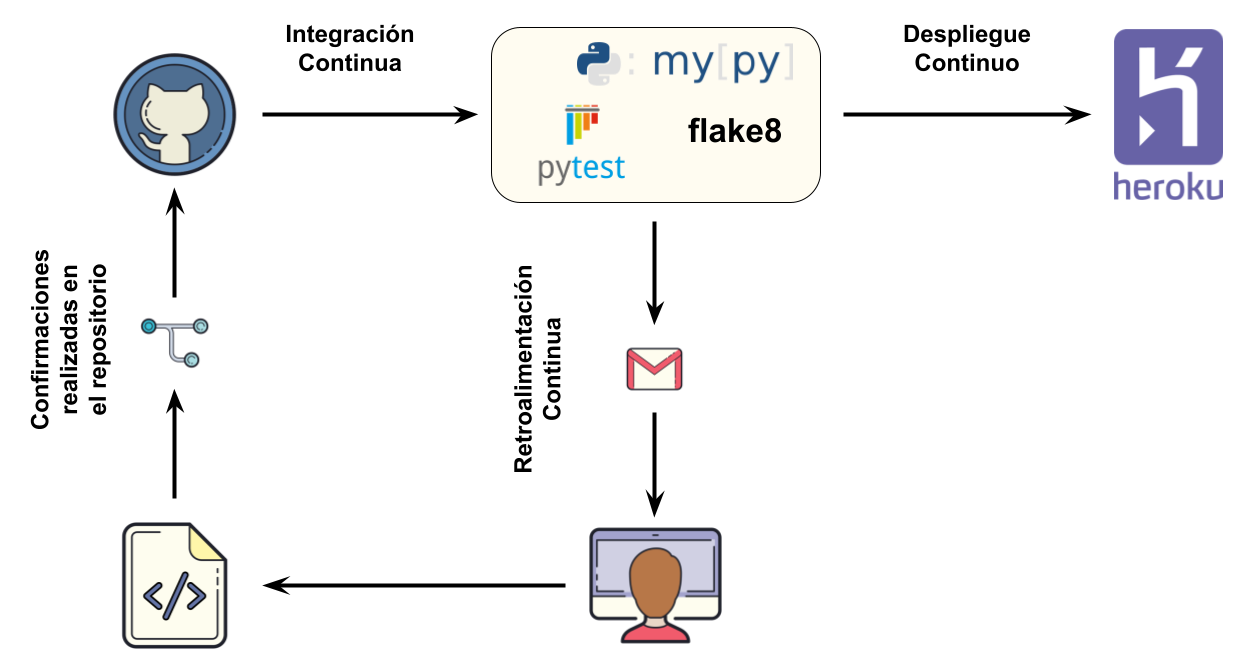
\includegraphics[width=0.95\textwidth]{gfx/CI-Diagram.png}
    \caption[Esquema \textit{DevOps} en el \textit{Back-end}]{Esquema \textit{DevOps} en el \textit{Back-end}.}\label{gfx:CI-Diagram}
\end{figure}

Cabe mencionar que cada herramienta tiene su propio archivo de configuración, al igual que \textit{GitHub Actions}, el cual se tiene que configurar mediante un archivo \ac{YAML} dentro de la carpeta \textit{.github/workflows}.

\section{Implementación Front-end}
Al igual que en la parte \textit{Back-end}, en esta capa también se ha usado un sistema de gestión de paquetes. Se ha usado el gestor de paquetes por defecto que ofrece Node.js, un entorno de ejecución para JavaScript, llamado \textit{npm}. Gracias a este gestor, podremos repetir y distribuir diferentes versiones del proyecto con el fin de cumplir las diferentes vías de \textit{DevOps}. \cite{npm-manual}

\vspace{0.2cm}

\begin{table}[H]
\centering
\small
\begin{tabular}{| >{\centering\arraybackslash}m{0.6in} >{\centering\arraybackslash}m{0.7in} |}
\hline
\multicolumn{1}{|p{0.6in}|}{\cellcolor{RoyalBlue}\textbf{Terminal:}} & \multicolumn{1}{p{0.7in}|}{\textit{npm install}} \\ \hline
\end{tabular}
\caption[Instalación del proyecto]{Instalación del proyecto.}
\end{table}

\begin{table}[H]
\centering
\small
\begin{tabular}{| >{\centering\arraybackslash}m{0.6in} >{\centering\arraybackslash}m{0.85in} |}
\hline
\multicolumn{1}{|p{0.6in}|}{\cellcolor{RoyalBlue}\textbf{Terminal:}} & \multicolumn{1}{p{0.85in}|}{\textit{npm run serve}} \\ \hline
\end{tabular}
\caption[Ejecución del proyecto]{Ejecución del proyecto.}
\end{table}

\begin{table}[H]
\centering
\small
\begin{tabular}{| >{\centering\arraybackslash}m{0.6in} >{\centering\arraybackslash}m{0.85in} |}
\hline
\multicolumn{1}{|p{0.6in}|}{\cellcolor{RoyalBlue}\textbf{Terminal:}} & \multicolumn{1}{p{0.85in}|}{\textit{npm run build}} \\ \hline
\end{tabular}
\caption[Construcción del proyecto]{Construcción del proyecto.}
\end{table}

En cuanto a las herramientas utilizadas para cumplir con la integración continua del proyecto fueron \textit{ESLint} y \textit{Prettier}. En primer lugar, \textit{ESLint} tiene como objetivo principal analizar el código y mostrar errores cometidos mediante reglas, las reglas que he escogido para ello son reglas predefinidas por el estándar de la compañía Airbnb, siendo este estándar un pilar dentro de la programación de JavaScript. \cite{eslint-manual}

\vspace{0.3cm}

Por otro lado, \textit{Prettier}  es un formateador de código obstinado, su función es ajustar el código mediante las reglas propuestas por el usuario. Ambas herramientas pueden llegar a coexistir e incluso beneficiarse de diferentes funciones que poseen.

\vspace{0.2cm}

\begin{table}[H]
\centering
\small
\begin{tabular}{| >{\centering\arraybackslash}m{0.6in} >{\centering\arraybackslash}m{0.8in} |}
\hline
\multicolumn{1}{|p{0.6in}|}{\cellcolor{RoyalBlue}\textbf{Terminal:}} & \multicolumn{1}{p{0.8in}|}{\textit{npm run lint}} \\ \hline
\end{tabular}
\caption[Ejecución del linter]{Ejecución del linter.}
\end{table}

Con ambas herramientas se termina consiguiendo una mejora de flujo de entrega e integración continua, ya que estas herramientas también son ejecutadas al realizar cambios y confirmaciones en el repositorio del código fuente. Además, se consigue un despliegue continuo gracias a la plataforma Vercel, ya que al igual que Heroku, también esta contactada con la plataforma de GitHub. Vercel también cumple con la retroalimentación continua, avisando por correo electrónico del estado del despliegue del proyecto.

\begin{figure}[H]
    \centering
    \myfloatalign
    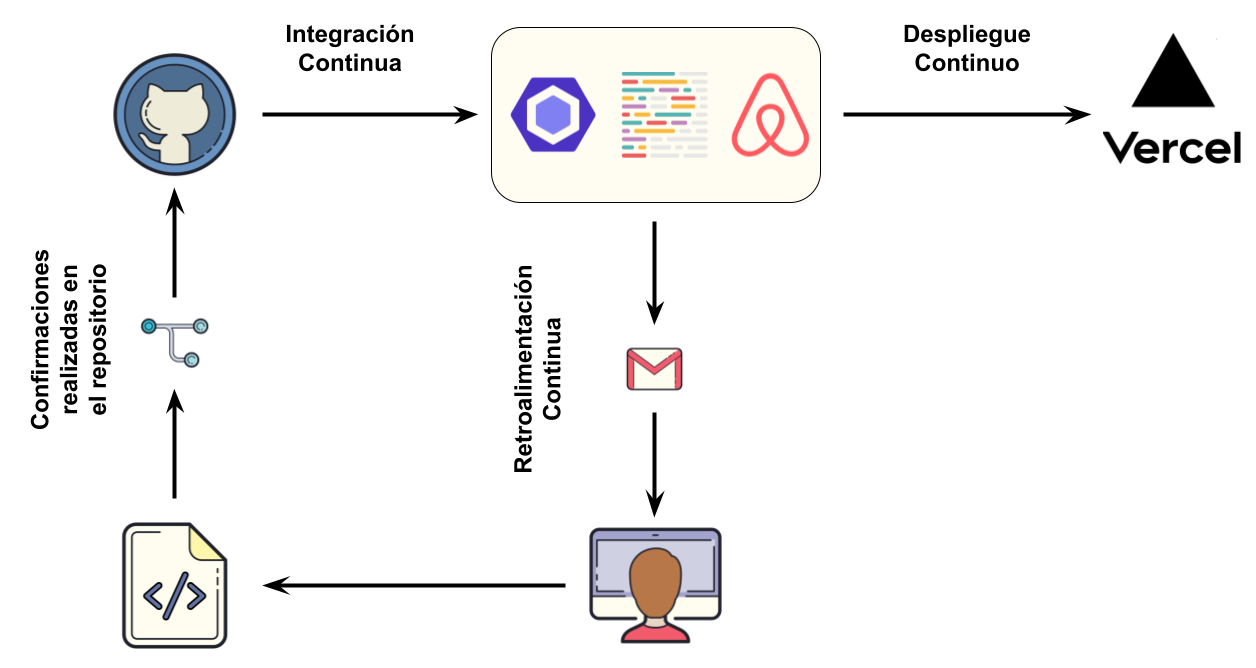
\includegraphics[width=0.95\textwidth]{gfx/CI-Diagram2.png}
    \caption[Esquema \textit{DevOps} en el \textit{Front-end}]{Esquema \textit{DevOps} en el \textit{Front-end}.}\label{gfx:CI-Diagram2}
\end{figure}
